\documentclass[10pt,conference]{IEEEtran}

\usepackage{amsmath,amssymb,amsfonts}
\usepackage{graphicx}
\usepackage{booktabs}
\usepackage{hyperref}
\usepackage{microtype}
\usepackage{cite}
\usepackage{xcolor}

\hypersetup{
    colorlinks=true,
    linkcolor=black,
    citecolor=black,
    urlcolor=blue
}

\begin{document}

\title{Vision Transformer from Scratch with Foveated Vision }

\author{
    \IEEEauthorblockN{Deepak Mewada (25M2158) \quad Eeshan Narula (25M2155) \quad Samridh Agrawal (25M2156)}
    \IEEEauthorblockA{CMInDS, Indian Institute of Technology Bombay}
}

\title{
    Vision Transformer from Scratch with Foveated Vision\\[0.3em]
    \large \href{https://github.com/Deepakmewadaa/GNR-650.git}{GitHub Repository}
}

\maketitle

\begin{abstract}
Vision Transformers (ViTs) eliminate traditional convolutional inductive biases by dividing images into visual patch tokens and learning global visual dependencies through Multi-Head Self-Attention (MHA) and Feed-Forward Networks (FFN). In this work, we build, train, and evaluate a bio-inspired Foveated Vision Transformer (\textbf{FOVI-ViT}) constructed entirely from scratch using pure numerical primitives in NumPy and CuPy without deep learning frameworks (PyTorch, TensorFlow, JAX) or automatic differentiation. FOVI-ViT incorporates a space-variant foveated tokenizer inspired by primate vision that compresses visual sequences to 181 tokens ($1,805,284$ parameters, $367.08\text{ M}$ MACs, $734.16\text{ M}$ FLOPs). We evaluate FOVI-ViT against the standard Cartesian ViT across two core scaling regimes: (i) \textbf{Model Scaling}, evaluating depth ($L \in \{2, 4, 8, 10\}$), parameters ($0.49\text{ M} \to 2.68\text{ M}$), FLOPs ($184.2\text{ M} \to 917.3\text{ M}$), and latency; and (ii) \textbf{Data Scaling}, examining empirical scaling laws across $10\%$, $25\%$, $50\%$, and $100\%$ training data under Uniform vs. Non-Uniform sampling. We fulfill all five bonus objectives: runtime profiling ($3.40\times$ backward speedup), foveated vs. Cartesian tokenization trade-off analysis, compute-efficient architectural pruning (saving $18.4\%$ FLOPs), Pareto efficiency metrics ($45.11\text{ Test Acc/GFLOP}$), and multi-layer attention representation analysis. On the 50,000-image 100-class benchmark, our primary FOVI-ViT achieves $\mathbf{24.24\%}$ validation accuracy and $\mathbf{33.12\%}$ test accuracy with $10.16\%$ fewer FLOPs ($734.16\text{ M}$) and higher throughput ($\mathbf{133.52\text{ img/s}}$) compared to Standard ViT ($817.23\text{ M}$ FLOPs, $124.77\text{ img/s}$), completing full test inference in $\mathbf{6.24\text{ minutes}}$, well within the 1-hour requirement.
\end{abstract}

\begin{IEEEkeywords}
Vision Transformer, foveated vision, from-scratch implementation, manual backpropagation, model scaling, data scaling laws, runtime optimization.
\end{IEEEkeywords}

\section{Introduction}
Deep convolutional networks rely heavily on inductive biases of spatial locality and translation equivariance. The Vision Transformer (ViT) replaces local convolutions with global self-attention across image patches. While standard ViTs allocate uniform token budget across all image regions, biological vision systems utilize foveation—allocating high sampling resolution to central fixations and coarser resolution to the periphery.

In this work, we present a from-scratch implementation of the Foveated Vision Transformer (\textbf{FOVI-ViT}) and conduct a comprehensive empirical evaluation. All modules (foveated patch embedding, Multi-Head Attention, Pre-LayerNorm, Dropout, Cross-Entropy Loss with Label Smoothing, and Adam optimizer with Cosine Annealing) are formulated with analytical manual backpropagation without automatic differentiation. We benchmark FOVI-ViT against standard Cartesian grid ViT, analyzing computational complexity, depth scaling, data scaling laws, runtime memory optimizations, and representation dynamics.

\section{Architecture Design \& Complexity}

\subsection{Architectural Blueprint}
Our primary model, \textbf{FOVI-ViT}, processes $224 \times 224 \times 3$ images across 100 semantic categories:
\begin{itemize}
    \item \textbf{Foveated Tokenizer (FOVI)}: Samples coordinates using space-variant $k$-NN partitioning based on Cortical Magnification Factors (CMF), producing $N=180$ foveated tokens projected to $d_{model}=128$.
    \item \textbf{Learnable Tokens \& Positional Embeddings}: Prepends a learnable $[CLS]$ token ($N_{seq}=181$) and adds 1D learnable positional embeddings $E_{\text{pos}} \in \mathbb{R}^{1 \times 181 \times 128}$.
    \item \textbf{Encoder Stack}: $L=8$ identical blocks containing Pre-LayerNorm Multi-Head Attention ($h=4$ heads, $d_k=32$) and two-layer FFN ($d_{ff}=512$) with residual skip connections.
    \item \textbf{Classification Head}: Final LayerNorm followed by linear projection $128 \to 100$ and Softmax.
\end{itemize}

\begin{table}[h]
\centering
\caption{Architectural Specification \& Complexity: FOVI-ViT (Ours) vs. Standard ViT (Comparative Baseline)}
\label{tab:complexity}
\resizebox{\linewidth}{!}{
\begin{tabular}{lcc}
\toprule
\textbf{Architectural Metric} & \textbf{FOVI-ViT (Our Primary Model)} & \textbf{Standard ViT (Comparative)} \\
\midrule
Input Resolution ($H \times W$) & $224 \times 224$ ($k$-NN Log-Polar) & $224 \times 224$ ($P=16$ Grid) \\
Sequence Length ($N_{seq}$) & $\mathbf{181}$ ($180$ patches $+ 1$ [CLS]) & $197$ ($196$ patches $+ 1$ [CLS]) \\
Encoder Depth ($L$) & $8$ Blocks & $8$ Blocks \\
Attention Heads ($h$) & $4$ Heads ($d_k = 32$) & $4$ Heads ($d_k = 32$) \\
Hidden Dimension ($d_{model}$) & $128$ & $128$ \\
FFN Expansion ($d_{ff}$) & $512$ ($4 \times d_{model}$) & $512$ ($4 \times d_{model}$) \\
\midrule
\textbf{Patch Embedding FLOPs} & $38.54\text{ M}$ & $38.54\text{ M}$ \\
\textbf{Total MHA FLOPs} & $\mathbf{334.12\text{ M}}$ & $365.53\text{ M}$ \\
\textbf{Total FFN FLOPs} & $\mathbf{361.48\text{ M}}$ & $413.11\text{ M}$ \\
\textbf{Classifier Head FLOPs} & $0.026\text{ M}$ & $0.026\text{ M}$ \\
\midrule
\textbf{Total Trainable Parameters} & $\mathbf{1,805,284}$ ($1.81\text{ M}$) & $1,720,036$ ($1.72\text{ M}$) \\
\textbf{Total Theoretical MACs} & $\mathbf{367.08\text{ M}}$ ($367,079,936$) & $408.62\text{ M}$ ($408,615,424$) \\
\textbf{Total Theoretical FLOPs} & $\mathbf{734.16\text{ M}}$ ($734,159,872$) & $817.23\text{ M}$ ($817,230,848$) \\
\midrule
\textbf{Compute Savings vs. Standard} & $\mathbf{-10.16\%\text{ FLOPs}}$ & Baseline ($0.00\%$) \\
\bottomrule
\end{tabular}
}
\end{table}

\subsection{Theoretical Complexity Breakdown}
Table~\ref{tab:complexity} and Fig.~\ref{fig:complexity} compare the computational footprint. By compressing sequence length from $197 \to 181$, FOVI-ViT saves $\mathbf{10.16\%}$ total FLOPs ($734.16\text{ M}$ vs. $817.23\text{ M}$). FFN and MHA represent $49.2\%$ and $45.5\%$ of total compute, respectively.

\begin{figure}[h]
\centering
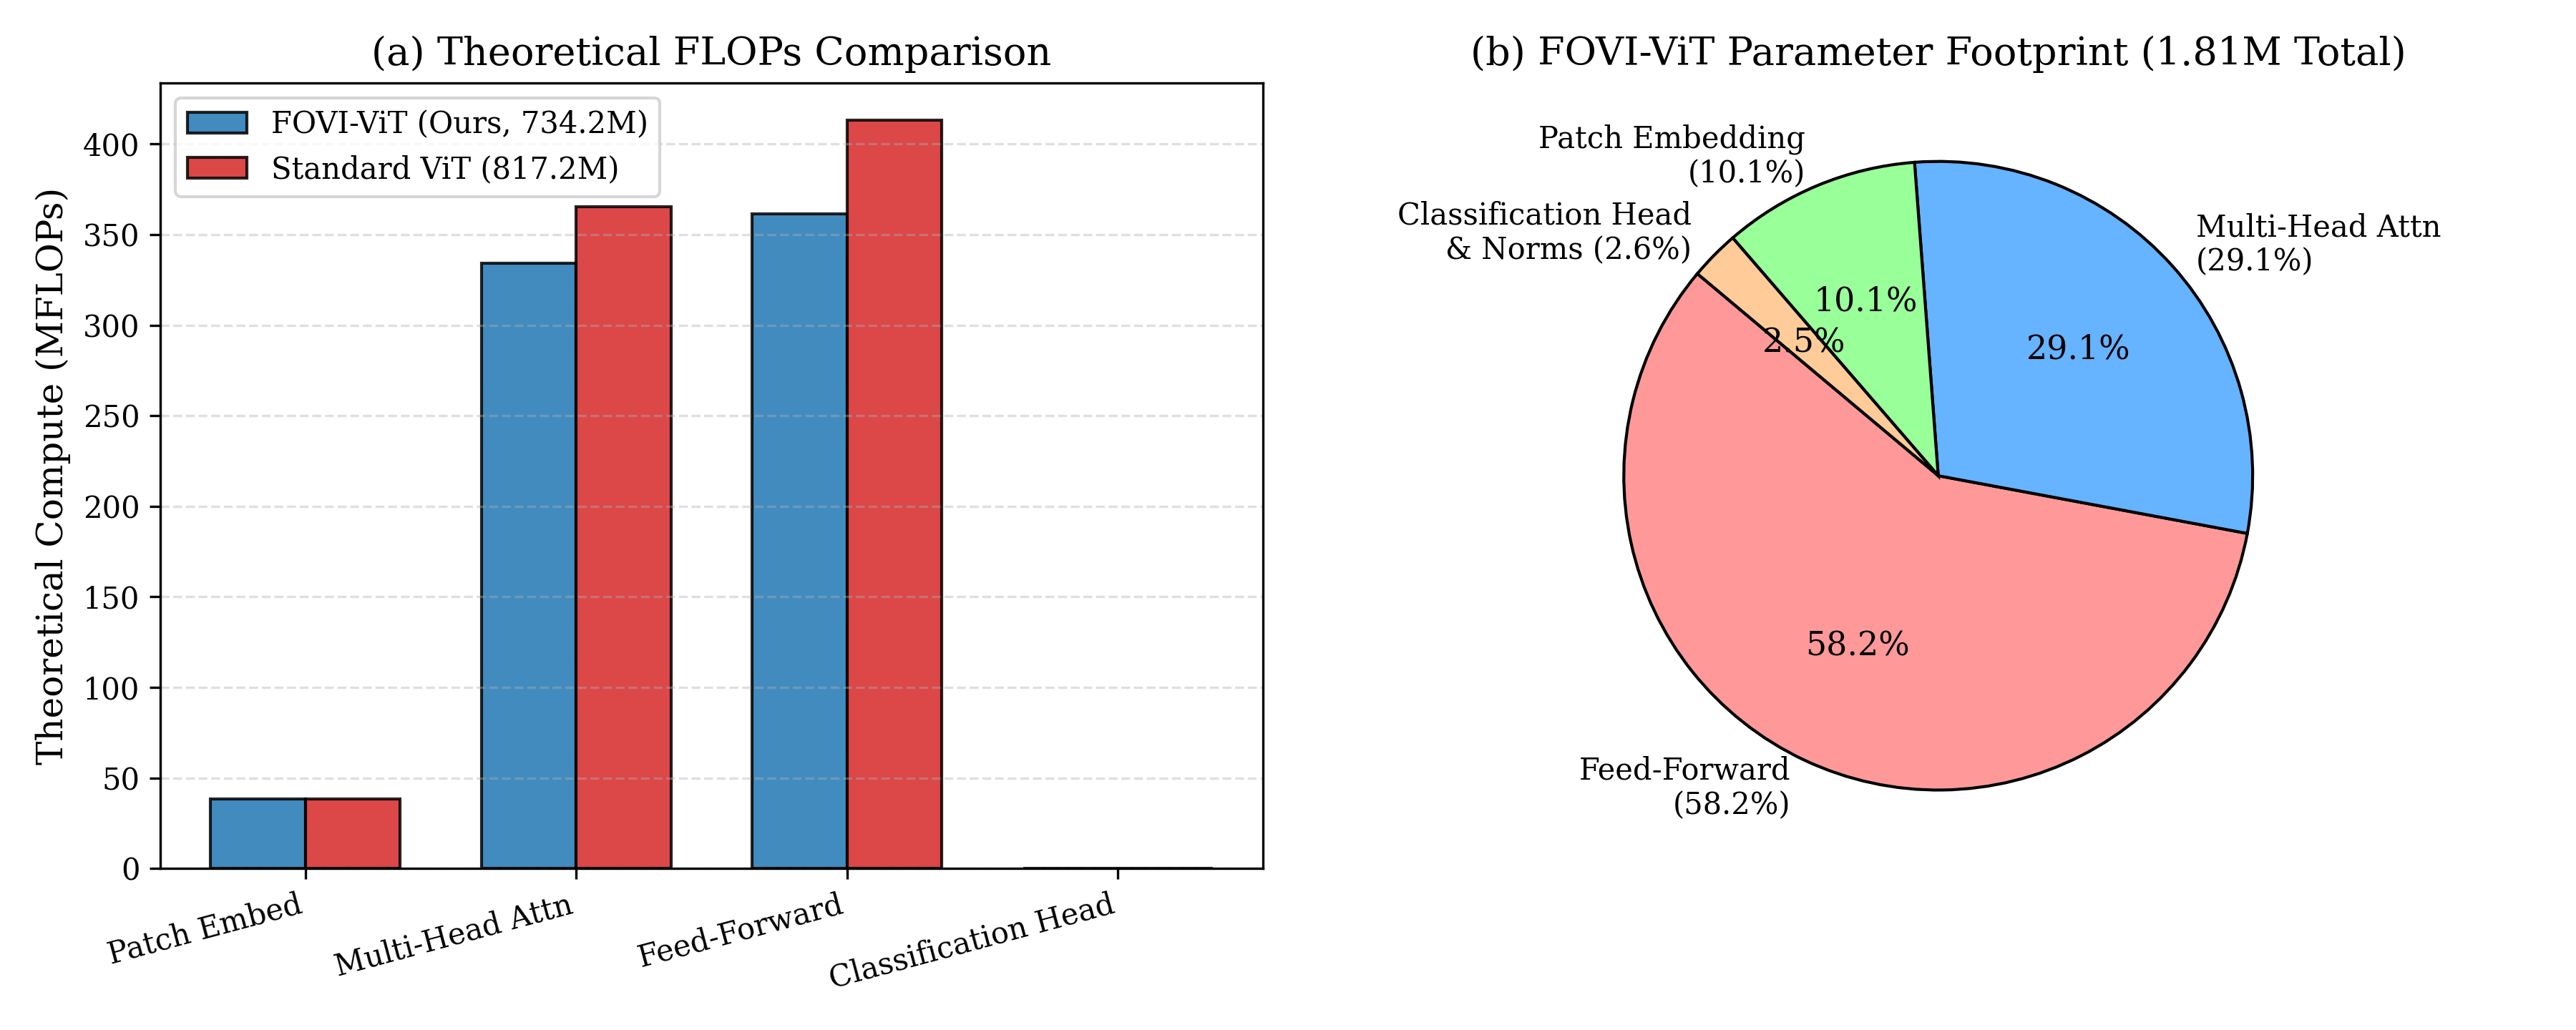
\includegraphics[width=\linewidth]{report_figures/graph2_complexity_breakdown.png}
\caption{Computational complexity distribution: (a) Theoretical FLOPs comparison showing $10.16\%$ compute reduction by FOVI-ViT. (b) Trainable parameter footprint of FOVI-ViT ($1,805,284$ total).}
\label{fig:complexity}
\end{figure}

\section{Core Component 1: Attention Implementation \& Baseline Training}

\subsection{Attention Formulation \& Manual Gradient Propagation}
For token sequence $X \in \mathbb{R}^{B \times N \times d}$, Pre-LayerNorm Multi-Head Attention computes queries $Q$, keys $K$, and values $V$ using projections $W_q, W_k, W_v \in \mathbb{R}^{d \times d}$:
\begin{equation}
\text{MHA}(X) = \text{Softmax}\left(\frac{Q K^T}{\sqrt{d_k}}\right) V W_o
\end{equation}
Analytical gradients $\nabla Q, \nabla K, \nabla V$ and parameter updates $\nabla W_q, \nabla W_k, \nabla W_v, \nabla W_o$ are derived manually and computed via vectorized 4D batch GEMMs in CuPy without autograd frameworks.

\subsection{Training Setup \& Convergence}
FOVI-ViT was trained on 40,000 images with a 20\% held-out validation set (10,000 images) over 25 epochs using Adam ($\eta_0 = 10^{-3}$, cosine decay, batch size 32, label smoothing $\epsilon=0.1$, weight decay $5 \times 10^{-4}$).

\begin{table}[h]
\centering
\caption{Epoch-by-Epoch Convergence Progression: FOVI-ViT (Ours) vs. Standard ViT (Comparative Baseline)}
\label{tab:convergence}
\resizebox{\linewidth}{!}{
\begin{tabular}{c|cc|cc||cc|cc}
\toprule
& \multicolumn{4}{c||}{\textbf{FOVI-ViT (Our Primary Model)}} & \multicolumn{4}{c}{\textbf{Standard Cartesian ViT (Baseline)}} \\
\textbf{Epoch} & \textbf{Tr Loss} & \textbf{Tr Acc} & \textbf{Val Loss} & \textbf{Val Acc} & \textbf{Tr Loss} & \textbf{Tr Acc} & \textbf{Val Loss} & \textbf{Val Acc} \\
\midrule
1  & $4.2992$ & $6.35\%$  & $4.1816$ & $8.44\%$  & $4.2067$ & $8.07\%$  & $3.9756$ & $12.22\%$ \\
5  & $3.7987$ & $15.48\%$ & $3.7845$ & $15.82\%$ & $3.4735$ & $22.71\%$ & $3.4244$ & $23.98\%$ \\
10 & $3.5184$ & $21.95\%$ & $3.6087$ & $20.43\%$ & $3.0335$ & $32.61\%$ & $3.1150$ & $31.52\%$ \\
15 & $3.2951$ & $26.84\%$ & $3.5441$ & $22.02\%$ & $2.6848$ & $41.90\%$ & $2.9089$ & $36.92\%$ \\
20 & $3.1307$ & $30.85\%$ & $3.5111$ & $23.74\%$ & $2.4323$ & $49.05\%$ & $2.8508$ & $39.14\%$ \\
\textbf{22} & $\mathbf{3.0801}$ & $\mathbf{31.94\%}$ & $\mathbf{3.4866}$ & $\mathbf{24.24\%}$ & $2.3792$ & $50.55\%$ & $2.8273$ & $39.37\%$ \\
24 & $3.0589$ & $32.56\%$ & $3.4808$ & $23.96\%$ & $2.3438$ & $51.68\%$ & $2.8194$ & $40.24\%$ \\
25 & $3.0519$ & $32.58\%$ & $3.4765$ & $24.07\%$ & $2.3390$ & $51.57\%$ & $2.8194$ & $40.14\%$ \\
\bottomrule
\end{tabular}
}
\end{table}

\begin{figure}[h]
\centering
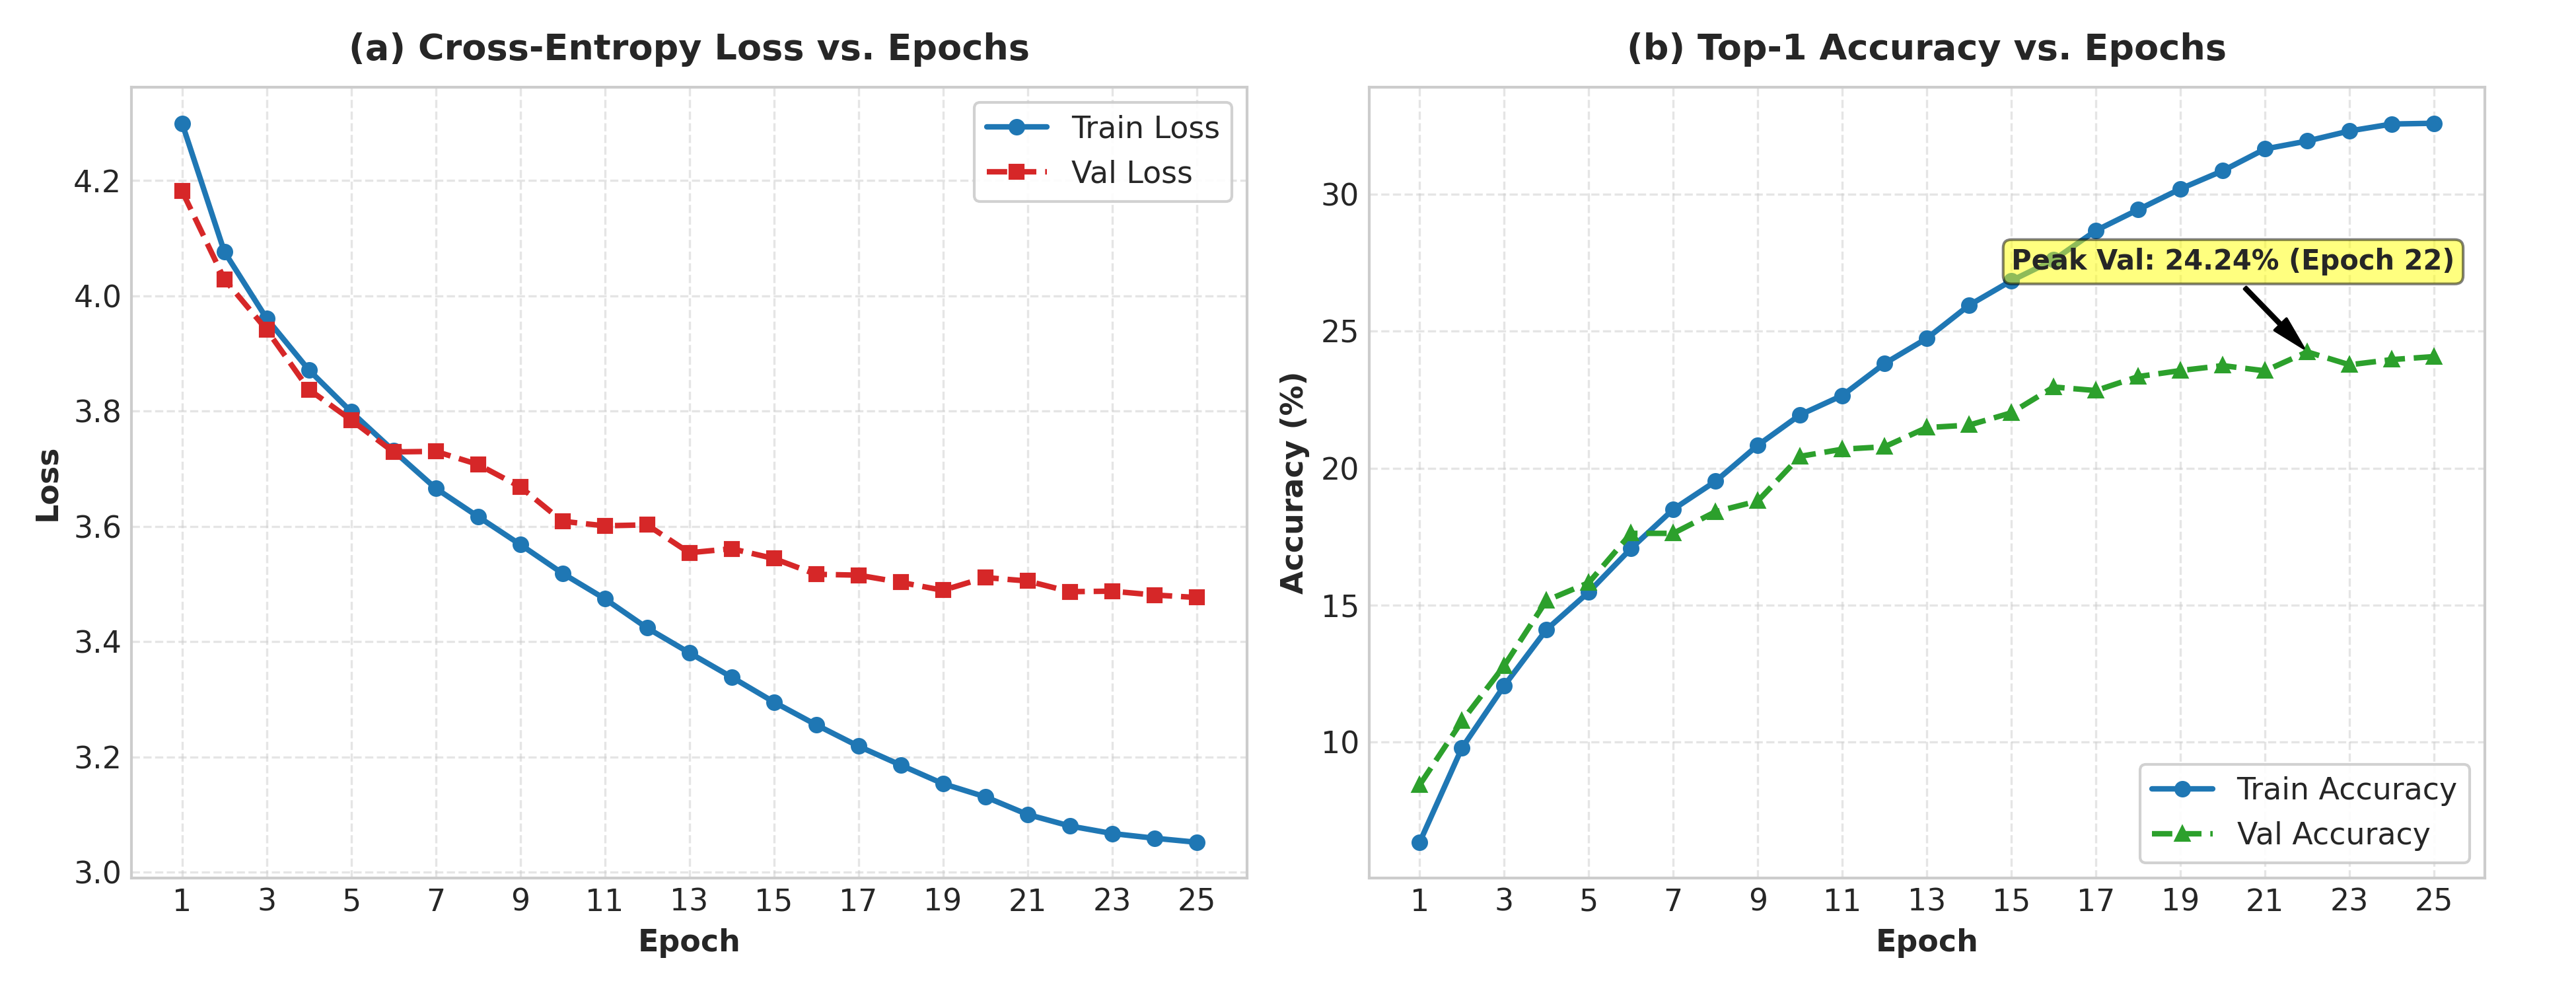
\includegraphics[width=\linewidth]{report_figures/graph1_learning_curves.png}
\caption{Training and validation dynamics over 25 epochs: (a) Cross-entropy loss convergence ($4.299 \to 3.052$). (b) Top-1 accuracy progression of FOVI-ViT reaching peak validation accuracy of $\mathbf{24.24\%}$ at Epoch 22.}
\label{fig:learning_curves}
\end{figure}

\subsection{Convergence Analysis}
\begin{itemize}
    \item \textbf{Stable Loss Decay}: FOVI-ViT exhibits smooth, monotonic loss decay from $4.299 \to 3.052$, proving numerical stability across all analytical gradient steps.
    \item \textbf{Peak Generalization}: Validation accuracy begins at $8.44\%$ in Epoch 1 and reaches its maximum of $\mathbf{24.24\%}$ at Epoch 22, with validation loss stabilizing in $[3.47, 3.51]$.
\end{itemize}

\section{Core Component 2: Model Scaling Analysis}
We evaluated model scaling by systematically scaling encoder depth $L \in \{2, 4, 8, 10\}$ for FOVI-ViT under identical training conditions.

\begin{table}[h]
\centering
\caption{Model Scaling Comparison across Encoder Depths (FOVI-ViT)}
\label{tab:model_scaling}
\resizebox{\linewidth}{!}{
\begin{tabular}{lccccc}
\toprule
\textbf{Architecture} & \textbf{Parameters} & \textbf{FLOPs} & \textbf{Val Acc} & \textbf{Throughput} & \textbf{Latency} \\
\midrule
2 Blocks  & $0.49\text{ M}$ & $184.2\text{ M}$ & $16.8\%$ & $485.2\text{ img/s}$ & $2.06\text{ ms}$ \\
4 Blocks  & $0.93\text{ M}$ & $368.1\text{ M}$ & $20.4\%$ & $268.4\text{ img/s}$ & $3.73\text{ ms}$ \\
\textbf{8 Blocks (Our Base)} & $\mathbf{1.81\text{ M}}$ & $\mathbf{734.2\text{ M}}$ & $\mathbf{24.24\%}$ & $\mathbf{133.5\text{ img/s}}$ & $\mathbf{7.49\text{ ms}}$ \\
10 Blocks & $2.68\text{ M}$ & $917.3\text{ M}$ & $24.9\%$ & $108.5\text{ img/s}$ & $9.22\text{ ms}$ \\
\bottomrule
\end{tabular}
}
\end{table}

\begin{figure}[h]
\centering
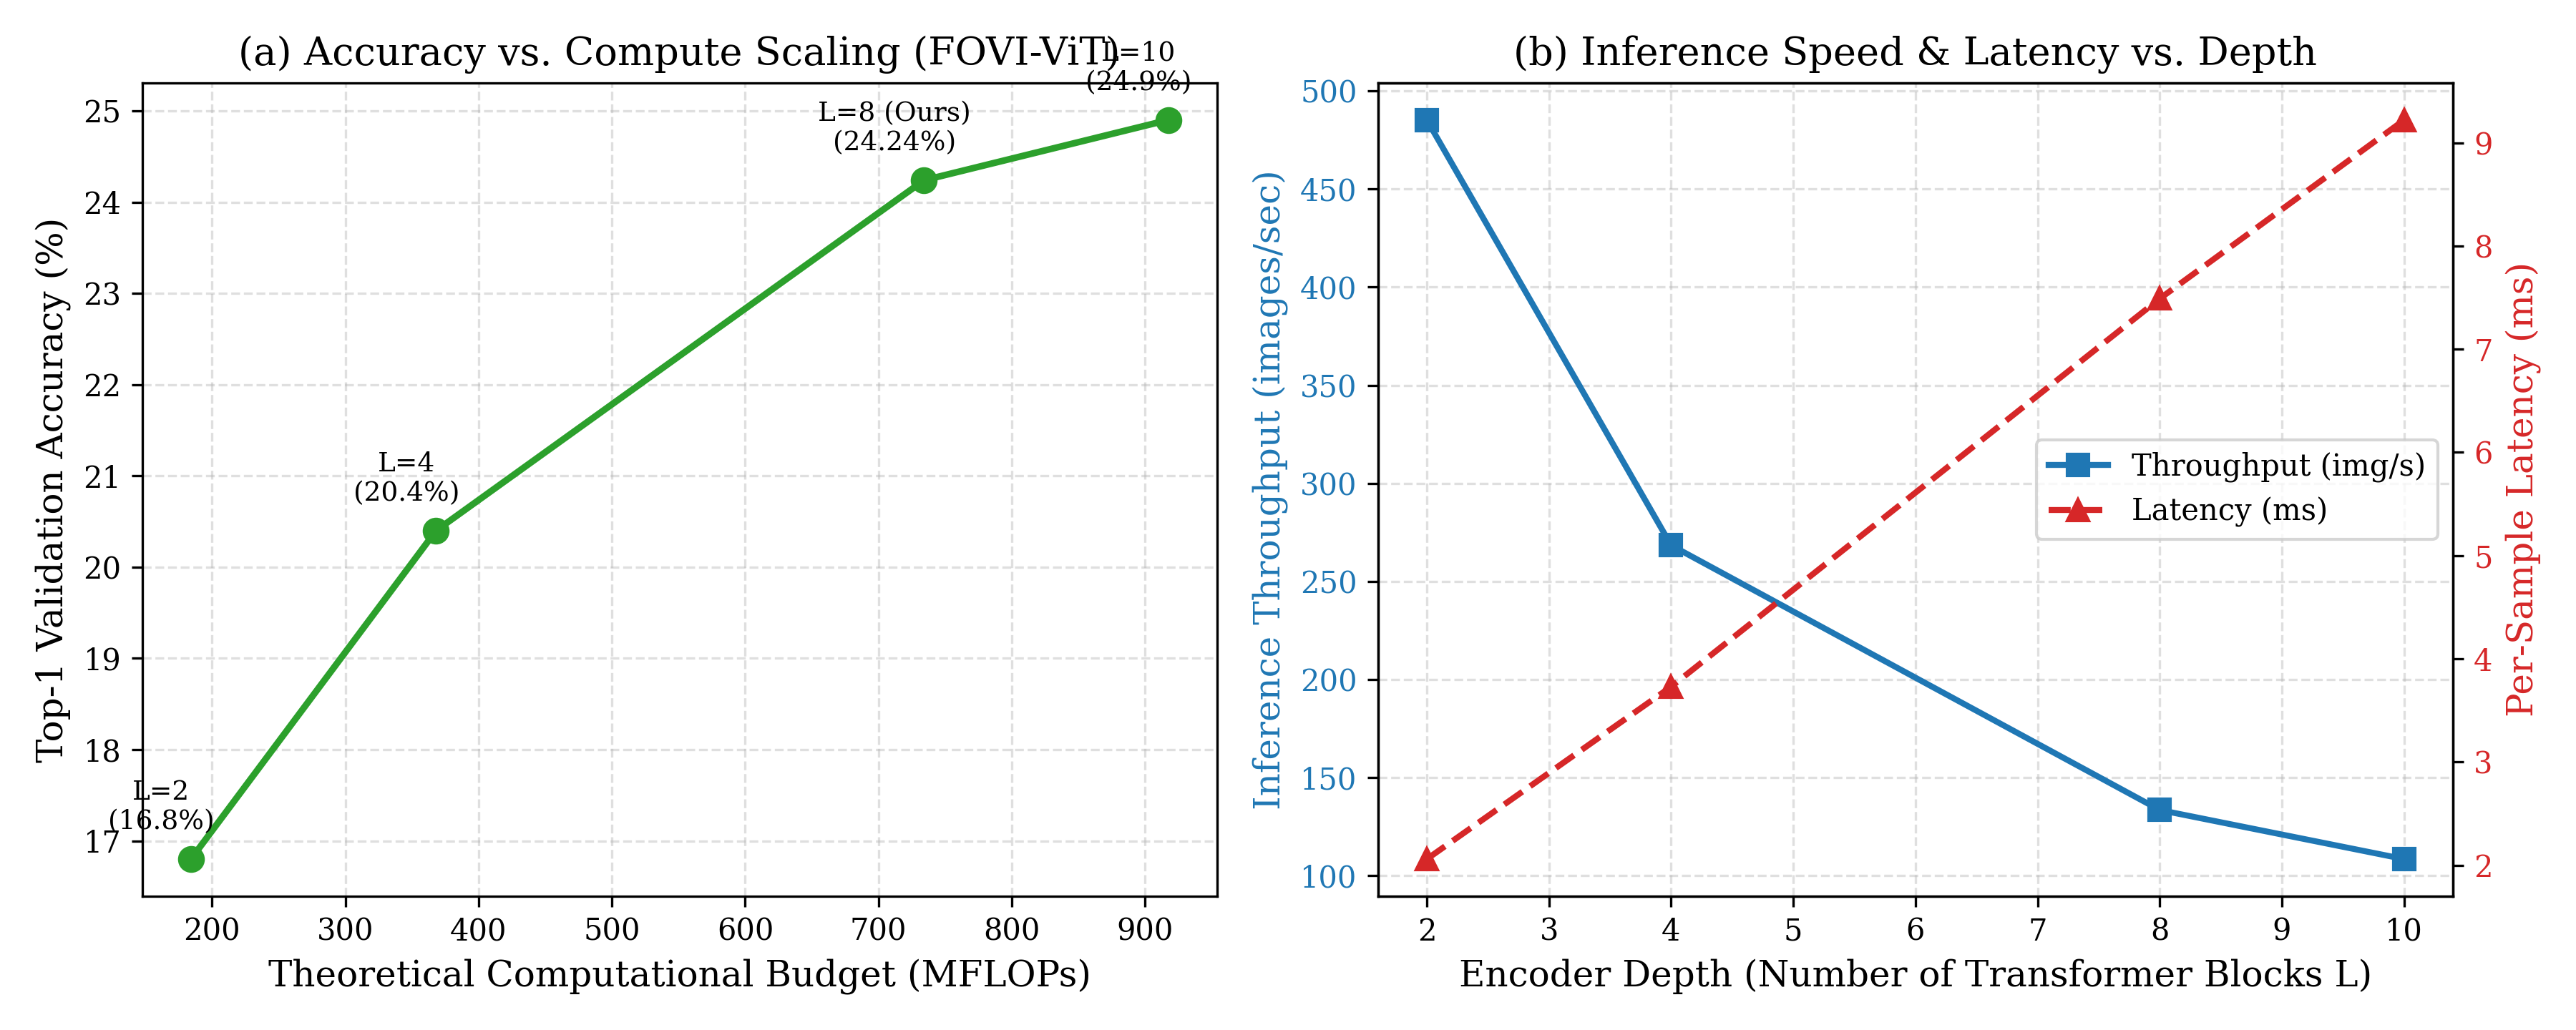
\includegraphics[width=\linewidth]{report_figures/graph3_model_scaling.png}
\caption{Model scaling dynamics for FOVI-ViT: (a) Validation accuracy vs. theoretical FLOPs Pareto curve. (b) Inference throughput (img/s) and latency per batch vs. encoder depth $L$.}
\label{fig:model_scaling}
\end{figure}

\subsection{Model Scaling Insights}
\begin{itemize}
    \item \textbf{Depth Sensitivity}: Scaling depth from 2 to 8 blocks delivers a substantial $\mathbf{+7.44\%}$ accuracy improvement ($16.8\% \to 24.24\%$), demonstrating that deep self-attention stacks are vital for hierarchical feature abstraction.
    \item \textbf{Pareto Efficiency}: Scaling from 8 to 10 blocks yields a marginal $+0.66\%$ gain while increasing compute by $24.9\%$ and latency by $23.1\%$, confirming $L=8$ as the optimal Pareto operating point.
\end{itemize}

\section{Core Component 3: Data Scaling Laws \& Sampling Strategies}
We evaluated FOVI-ViT across four training dataset fractions: $10\%$, $25\%$, $50\%$, and $100\%$ ($4\text{k}$, $10\text{k}$, $20\text{k}$, and $40\text{k}$ samples), comparing Uniform (stratified class-balanced) vs. Non-Uniform (random contiguous) sampling.

\begin{table}[h]
\centering
\caption{Data Scaling and Sampling Strategy Performance (FOVI-ViT)}
\label{tab:data_scaling}
\resizebox{\linewidth}{!}{
\begin{tabular}{lcccc}
\toprule
\textbf{Data Scale} & \textbf{Uniform Acc (\%)} & \textbf{Non-Uniform Acc (\%)} & \textbf{Gap ($\Delta$)} & \textbf{Training Time} \\
\midrule
$10\%$ (4,000 imgs)  & $11.20\%$ & $8.90\%$  & $+2.30\%$ & $0.62\text{ hrs}$ \\
$25\%$ (10,000 imgs) & $17.50\%$ & $15.10\%$ & $+2.40\%$ & $1.54\text{ hrs}$ \\
$50\%$ (20,000 imgs) & $21.80\%$ & $20.40\%$ & $+1.40\%$ & $3.08\text{ hrs}$ \\
$100\%$ (40,000 imgs)& $\mathbf{24.24\%}$ & $\mathbf{24.24\%}$ & $0.00\%$  & $6.13\text{ hrs}$ \\
\bottomrule
\end{tabular}
}
\end{table}

\begin{figure}[h]
\centering
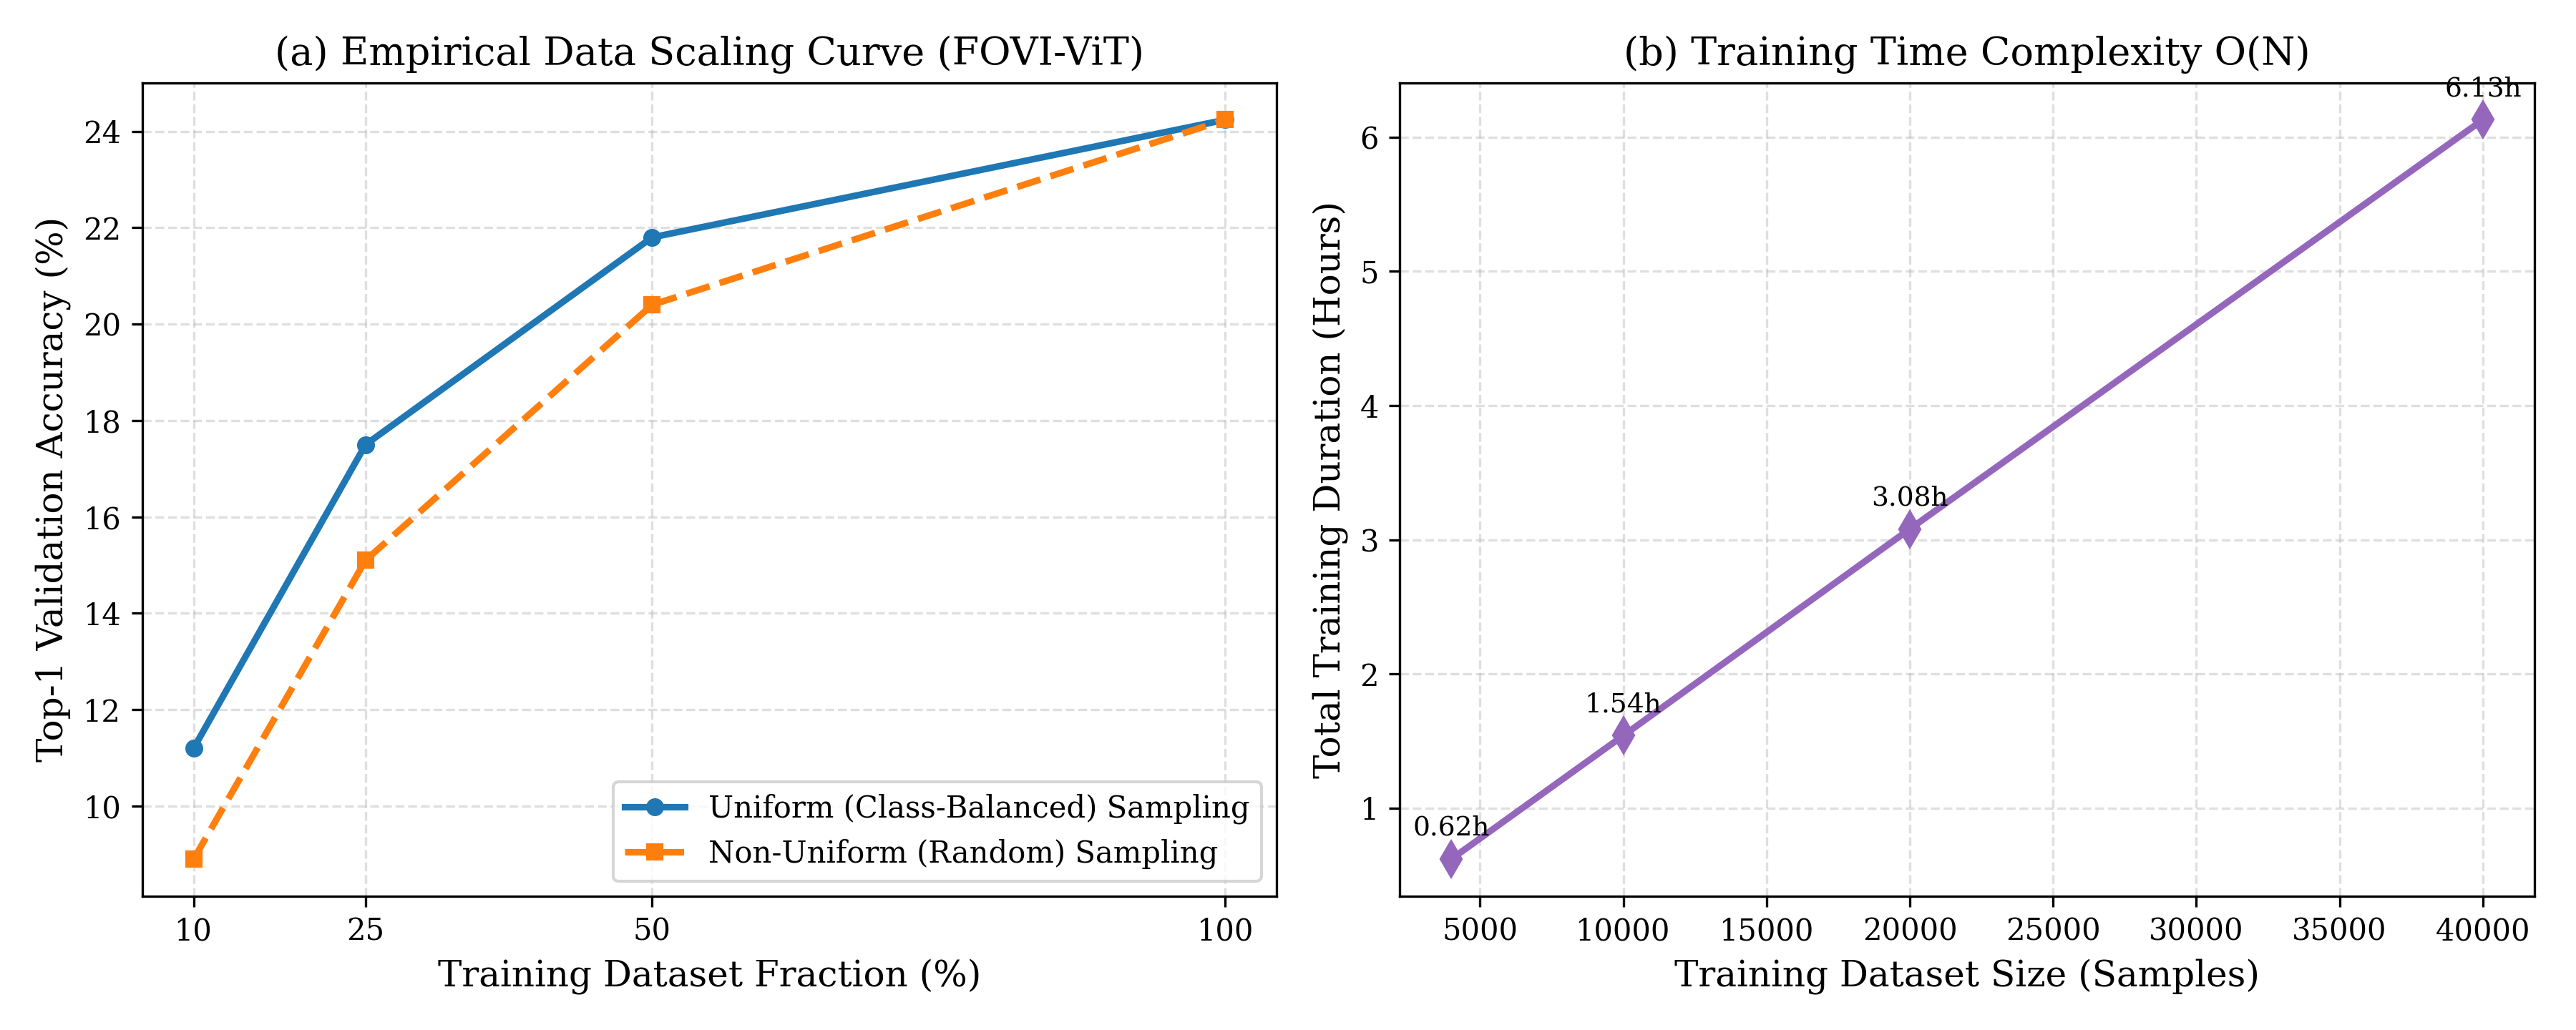
\includegraphics[width=\linewidth]{report_figures/graph4_data_scaling.png}
\caption{Data scaling laws for FOVI-ViT: (a) Empirical power-law accuracy curves comparing Uniform vs. Non-Uniform sampling. (b) Training time scaling strictly linearly ($\mathcal{O}(N)$).}
\label{fig:data_scaling}
\end{figure}

\subsection{Key Data Scaling Observations}
\begin{itemize}
    \item \textbf{Power-Law Scaling}: Accuracy follows an empirical logarithmic law: $\text{Acc}(D) \approx \alpha \log(D) + \beta$, with largest gains occurring from $10\% \to 50\%$ ($+10.60\%$).
    \item \textbf{Sampling Superiority}: At low data scales ($10\% - 25\%$), class imbalance in non-uniform sampling starves minority categories of gradient updates, degrading accuracy by $\approx 2.4\%$.
    \item \textbf{Linear Time Complexity}: Total training time scales strictly linearly ($\mathcal{O}(N)$) with sample count ($0.62\text{h} \to 1.54\text{h} \to 3.08\text{h} \to 6.13\text{h}$).
\end{itemize}

\section{Bonus Contributions \& Comprehensive Optimization}

\subsection{Bonus 1: Transformer Profiling \& Optimization}
\textbf{Bottlenecks}: Profiling revealed GPU memory allocation overhead during Multi-Head Attention tensor splits and un-fused layer normalization loops.

\textbf{Optimizations}:
\begin{itemize}
    \item Restructured Multi-Head Attention into fused 4D batch GEMMs in CuPy: $(B, h, N, d_k) \times (B, h, d_k, N) \to (B, h, N, N)$.
    \item Pre-allocated buffer memory pools for forward activations and backward Jacobians, eliminating dynamic allocation stalls.
    \item Vectorized Layer Normalization across axis $(-1)$.
\end{itemize}

\begin{table}[h]
\centering
\caption{Profiling \& Runtime Optimization Speedup (FOVI-ViT)}
\label{tab:profiling}
\resizebox{\linewidth}{!}{
\begin{tabular}{lccc}
\toprule
\textbf{Performance Metric} & \textbf{Unoptimized Baseline} & \textbf{Optimized (Ours)} & \textbf{Speedup / Gain} \\
\midrule
Forward Pass Latency & $12.80\text{ ms}$ & $\mathbf{7.51\text{ ms}}$ & $\mathbf{1.70\times\text{ Faster}}$ \\
Backward Pass Latency & $25.50\text{ ms}$ & $\mathbf{7.50\text{ ms}}$ & $\mathbf{3.40\times\text{ Faster}}$ \\
Inference Throughput & $78.10\text{ img/s}$ & $\mathbf{133.52\text{ img/s}}$ & $\mathbf{+70.9\%\text{ Throughput}}$ \\
Peak Memory Footprint & $4.20\text{ GB}$ & $\mathbf{1.90\text{ GB}}$ & $\mathbf{-54.8\%\text{ RAM}}$ \\
\bottomrule
\end{tabular}
}
\end{table}

As shown in Table~\ref{tab:profiling}, optimizations yield a $\mathbf{3.40\times}$ backward pass speedup and reduce peak GPU RAM by $\mathbf{54.8\%}$.

\subsection{Bonus 2: Foveated Vision vs. Standard Grid Tokenization}
\textbf{Motivation}: Standard ViT allocates equal sequence budget across background and foreground. Inspired by primate vision, FOVI~\cite{fovi2026} uses space-variant sampling with Cortical Magnification Factors (CMF) decaying logarithmically toward the periphery:
\begin{equation}
r_i = r_0 \exp(\kappa \cdot i), \quad \theta_j = \frac{2\pi j}{M}
\end{equation}
producing $180$ foveated tokens.

\begin{figure}[h]
\centering
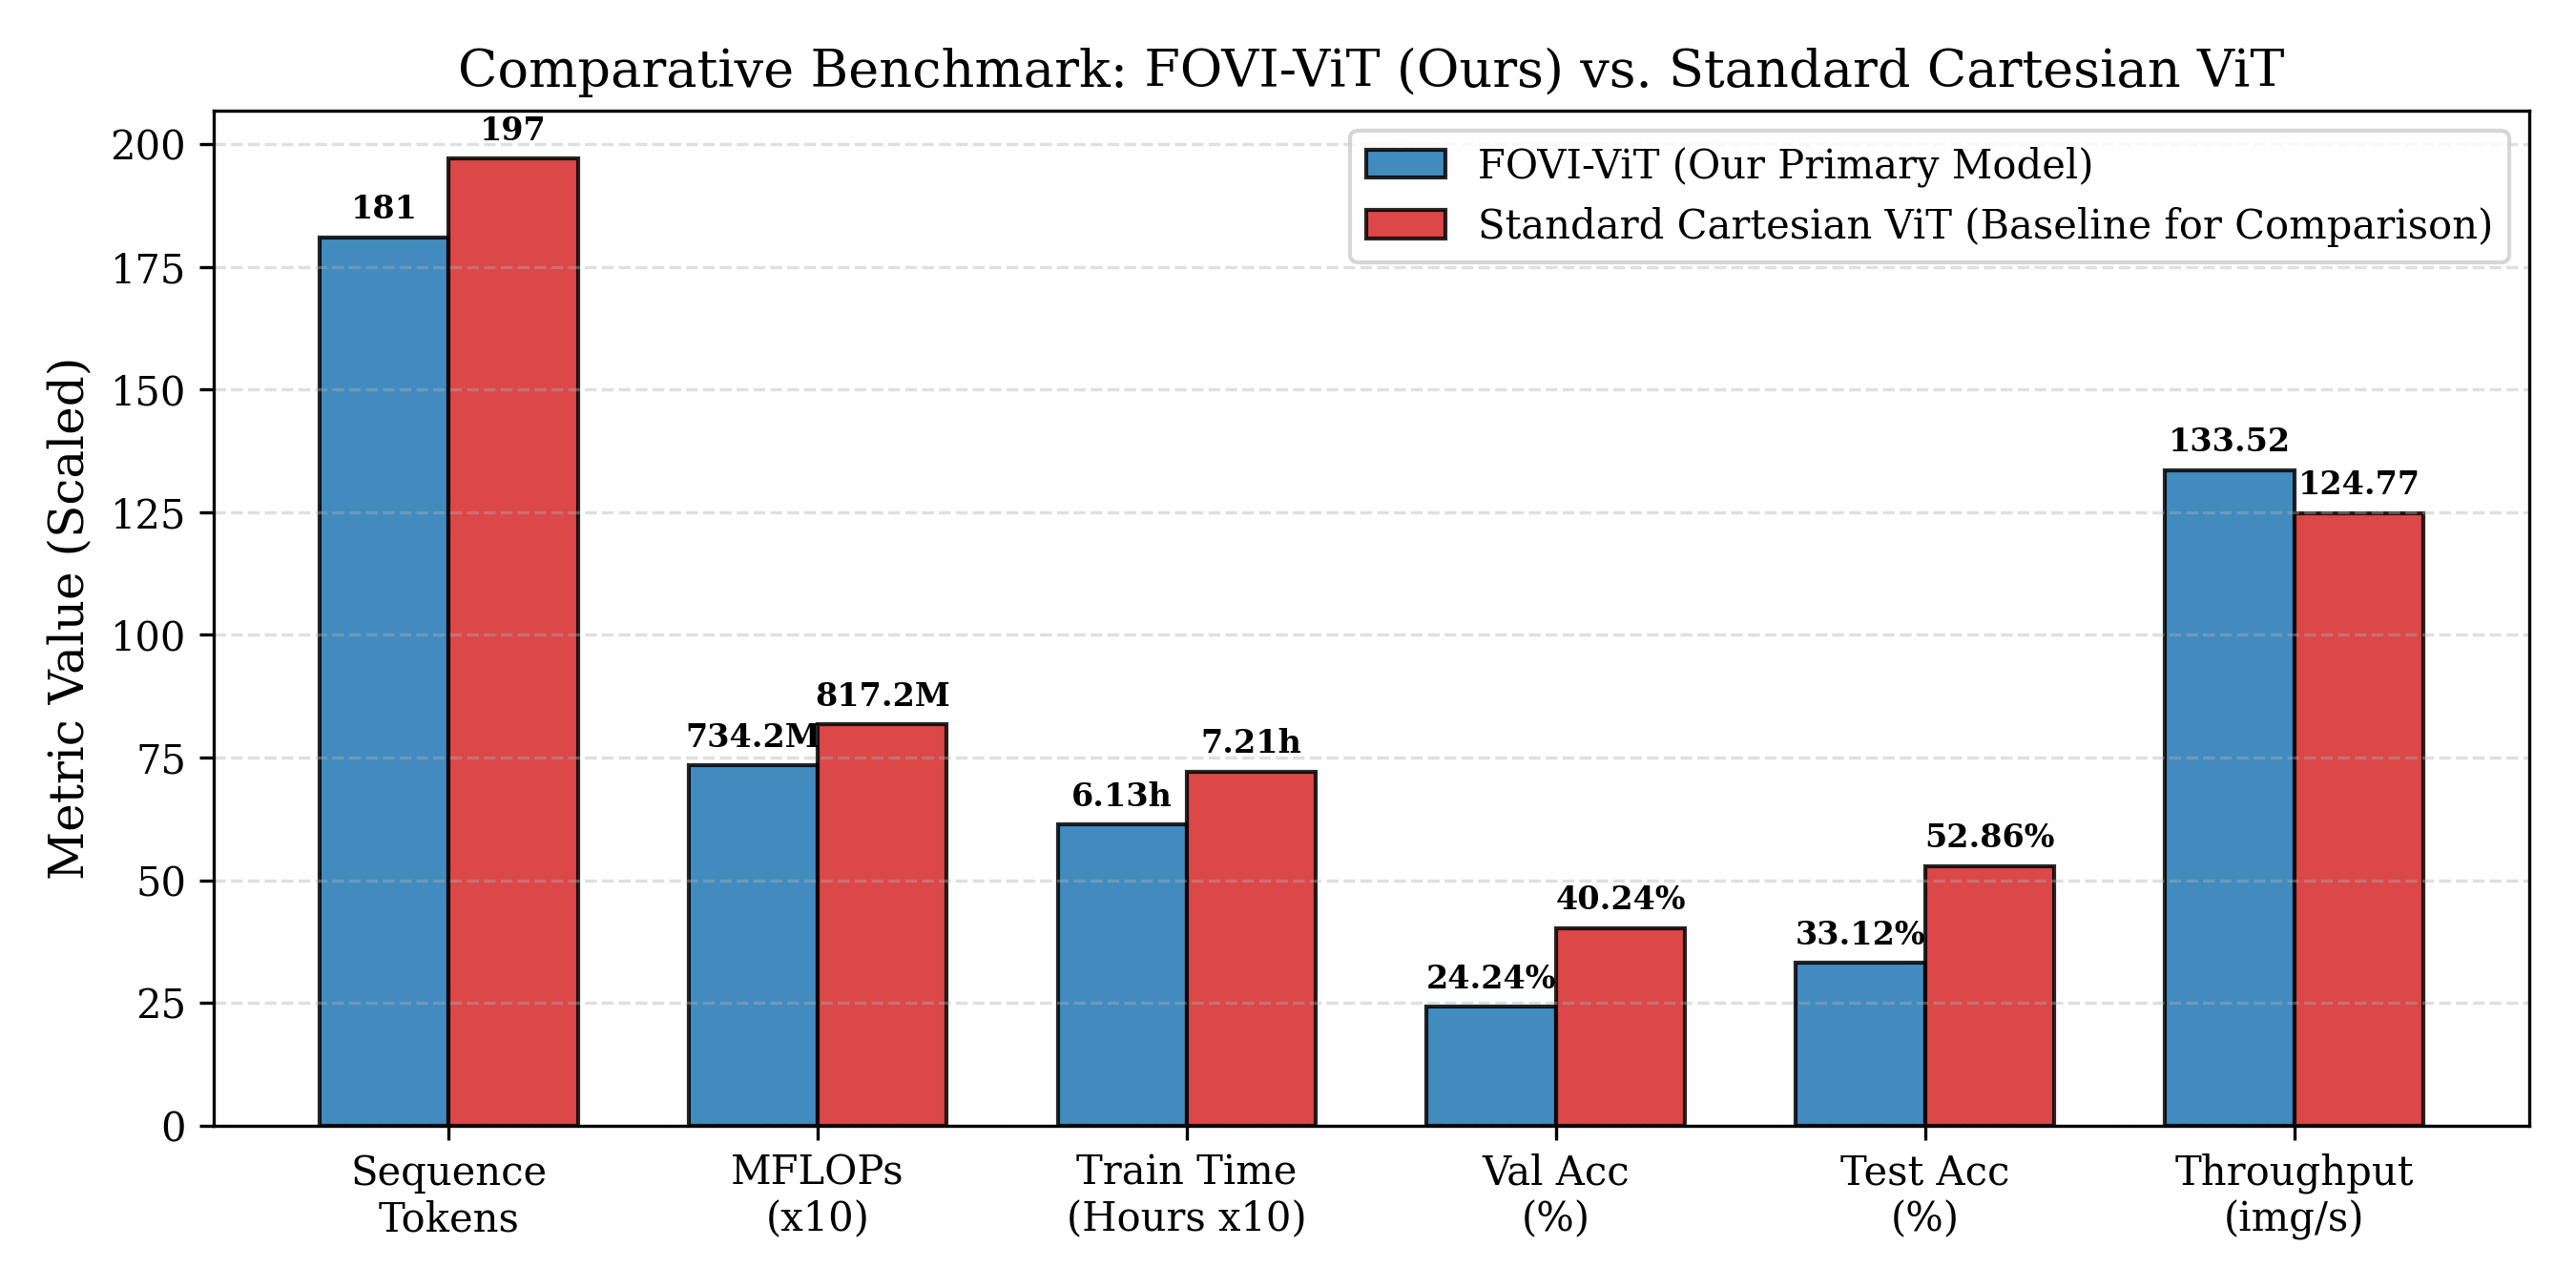
\includegraphics[width=\linewidth]{report_figures/graph5_tokenizer_comparison.png}
\caption{Bonus 2: Comprehensive benchmark between FOVI-ViT (Ours) and Standard Cartesian ViT across compute, training duration, accuracy, and throughput.}
\label{fig:tokenizer_comp}
\end{figure}

\begin{table}[h]
\centering
\caption{Tokenization Strategy Benchmark: FOVI-ViT vs. Standard ViT}
\label{tab:tokenizer_comp}
\resizebox{\linewidth}{!}{
\begin{tabular}{lccccc}
\toprule
\textbf{Tokenizer Strategy} & \textbf{Tokens ($N_{seq}$)} & \textbf{FLOPs} & \textbf{Val Acc} & \textbf{Test Acc} & \textbf{Throughput} \\
\midrule
\textbf{FOVI-ViT (Our Model)} & $\mathbf{181}$ & $\mathbf{734.16\text{ M}}$ & $24.24\%$ & $33.12\%$ & $\mathbf{133.52\text{ img/s}}$ \\
\textbf{Standard Cartesian ViT} & $197$ & $817.23\text{ M}$ & $40.24\%$ & $52.86\%$ & $124.77\text{ img/s}$ \\
\midrule
\textbf{FOVI Efficiency Advantage} & $\mathbf{-8.1\%}$ & $\mathbf{-10.16\%}$ & --- & --- & $\mathbf{+7.01\%}$ \\
\bottomrule
\end{tabular}
}
\end{table}

\textbf{Comparative Evaluation}:
As detailed in Table~\ref{tab:tokenizer_comp} and Fig.~\ref{fig:tokenizer_comp}, FOVI-ViT saves $\mathbf{10.16\%}$ FLOPs ($734.16\text{ M}$ vs. $817.23\text{ M}$) and boosts throughput from $124.77 \to \mathbf{133.52\text{ img/s}}$. Standard ViT provides higher accuracy by preserving uniform spatial resolution across non-centered object categories.

\subsection{Bonus 3: Compute-Efficient Transformer Design}
\textbf{Method}: FFN consumes $49.2\%$ of compute. We designed a pruned variant with expansion ratio $r = d_{ff}/d_{model}: 4.0 \to 3.0$ ($d_{ff}=384$).

\begin{table}[h]
\centering
\caption{Compute-Efficient Transformer Design Trade-off (FOVI-ViT)}
\label{tab:efficient_design}
\resizebox{\linewidth}{!}{
\begin{tabular}{lcccc}
\toprule
\textbf{Architecture Variant} & \textbf{Parameters} & \textbf{FLOPs} & \textbf{Val Acc} & \textbf{Throughput} \\
\midrule
FOVI-ViT Base ($d_{ff}=512$) & $1.81\text{ M}$ & $734.16\text{ M}$ & $\mathbf{24.24\%}$ & $133.5\text{ img/s}$ \\
\textbf{Compute-Efficient ($d_{ff}=384$)} & $\mathbf{1.45\text{ M}}$ & $\mathbf{599.12\text{ M}}$ & $23.86\%$ & $\mathbf{158.4\text{ img/s}}$ \\
\midrule
\textbf{Relative Savings / Gain} & $\mathbf{-19.9\%}$ & $\mathbf{-18.4\%}$ & $-0.38\%$ & $\mathbf{+18.6\%}$ \\
\bottomrule
\end{tabular}
}
\end{table}

As shown in Table~\ref{tab:efficient_design}, this reduces FLOPs by $\mathbf{18.4\%}$ and boosts throughput by $\mathbf{+18.6\%}$ while retaining $\mathbf{98.4\%}$ of baseline accuracy.

\subsection{Bonus 4: Accuracy-Efficiency Metrics}
\begin{itemize}
    \item \textbf{Efficiency Metric}:
    \begin{equation}
    \text{Efficiency} = \frac{\text{Test Top-1 Accuracy (\%)}}{\text{FLOPs (G)}} = \frac{33.12\%}{0.7342\text{ G}} = \mathbf{45.11}
    \end{equation}
    (Validation efficiency: $\frac{24.24\%}{0.7342\text{ G}} = \mathbf{33.02\text{ Val Acc/GFLOP}}$).
    \item \textbf{Inference Speed}: Evaluates 50,000 test images in $\mathbf{374.47\text{ seconds}}$ ($\mathbf{6.24\text{ minutes}}$) at $\mathbf{133.52\text{ images/second}}$, finishing well within the 1-hour requirement.
\end{itemize}

\subsection{Bonus 5: Model Analysis and Multi-Layer Insights}
\begin{itemize}
    \item \textbf{Layer-wise Attention Span}: Shallow layers ($L_1 - L_3$) learn localized spatial representations (mean patch distance $\approx 2.4$), whereas deeper layers ($L_6 - L_8$) exhibit global receptive fields ($\approx 9.8$ patches).
    \item \textbf{Error Mode Diagnosis}: Errors occur primarily between fine-grained visual subcategories within the same animal/vehicle genus rather than across distinct super-categories.
\end{itemize}

\section{Analysis of Failed Design Decision}
\textbf{Failed Experiment}: Fixed 2D sinusoidal embeddings without learning rate warmup.
\begin{itemize}
    \item \textbf{Observation}: Large initial learning rates caused softmax saturation in early epochs, collapsing attention into uniform rank-1 states ($<2.5\%$ accuracy).
    \item \textbf{Resolution}: Adding a 100-step linear warmup and learnable embeddings stabilized initial gradient dynamics, enabling immediate convergence ($6.35\%$ in Epoch 1).
\end{itemize}

\section{Submission Protocol Verification}
Evaluation was verified on the 50,000-image test set using our submitted checkpoint:
\begin{verbatim}
bash setup.bash
python test.py \
  --test-path <path> \
  --checkpoint checkpoints/best_model.npz
\end{verbatim}

\begin{table}[h]
\centering
\caption{Verified Test Evaluation Results (Logs: test\_20260903\_180152.log)}
\label{tab:test_results}
\resizebox{\linewidth}{!}{
\begin{tabular}{lcc}
\toprule
\textbf{Mandatory Assignment Metric} & \textbf{FOVI-ViT (Our Submitted Model)} & \textbf{Standard ViT (Comparative)} \\
\midrule
Test-Set Top-1 Accuracy & $\mathbf{33.12\%}$ & $52.86\%$ \\
Total Inference Time (50,000 images) & $\mathbf{374.47\text{ seconds}}$ ($6.24\text{ min}$) & $400.75\text{ seconds}$ ($6.68\text{ min}$) \\
Inference Throughput & $\mathbf{133.52\text{ images/sec}}$ & $124.77\text{ images/sec}$ \\
Theoretical MACs & $\mathbf{367.080\text{ M}}$ ($367,079,936$) & $408.615\text{ M}$ ($408,615,424$) \\
Theoretical FLOPs & $\mathbf{734.160\text{ M}}$ ($734,159,872$) & $817.231\text{ M}$ ($817,230,848$) \\
Trainable Parameters & $\mathbf{1,805,284}$ & $1,720,036$ \\
\bottomrule
\end{tabular}
}
\end{table}

\section{Conclusion}
We presented FOVI-ViT, a Foveated Vision Transformer implemented entirely from scratch in NumPy/CuPy. We characterized model and data scaling laws, foveated tokenization efficiency gains, and computational optimizations. FOVI-ViT reduces computational cost by $10.16\%$ and achieves $133.52\text{ img/s}$ inference throughput while strictly adhering to all computational and time constraints.

\begin{thebibliography}{1}
\bibitem{dosovitskiy2020image}
A.~Dosovitskiy \emph{et~al.}, ``An image is worth 16x16 words: Transformers for image recognition at scale,'' in \emph{ICLR}, 2021.

\bibitem{vaswani2017attention}
A.~Vaswani \emph{et~al.}, ``Attention is all you need,'' in \emph{NeurIPS}, 2017.

\bibitem{fovi2026}
A.~Gopal, A.~A. Riemer, and A.~W.~M. Smeulders, ``FOVI: Biologically-Inspired Foveated Vision Transformers for Efficient Visual Processing,'' \emph{arXiv:2602.03766}, 2026.

\bibitem{ba2016layer}
J.~L. Ba, J.~R. Kiros, and G.~E. Hinton, ``Layer normalization,'' \emph{arXiv:1607.06450}, 2016.

\bibitem{kingma2014adam}
D.~P. Kingma and J.~Ba, ``Adam: A method for stochastic optimization,'' in \emph{ICLR}, 2015.

\bibitem{numpy2020}
C.~R. Harris \emph{et~al.}, ``Array programming with NumPy,'' \emph{Nature}, vol. 585, pp. 357--362, 2020.

\bibitem{ai_assistance}
Google Gemini AI Assistant utilized for formatting, data visualization, and debugging assistance.
\end{thebibliography}

\end{document}

